\documentclass[border=10pt]{standalone}
\usepackage{pgfplots}
\pgfplotsset{compat=1.18}

\begin{document}

% Cross-section 1: y = 1 (circle in xz-plane)
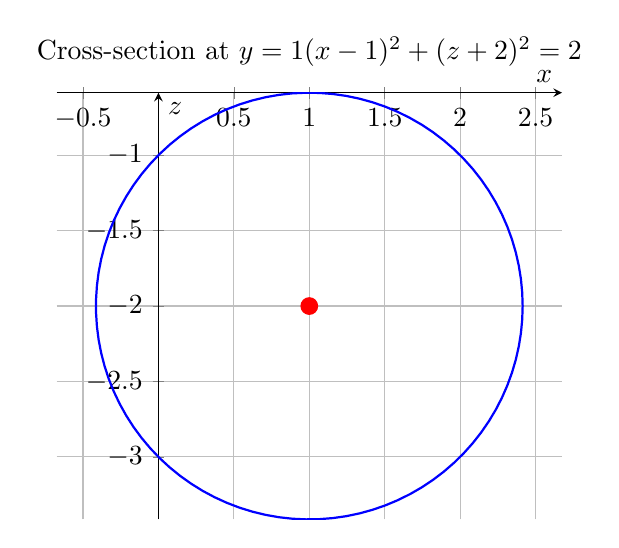
\begin{tikzpicture}
\begin{axis}[
    width=8cm,
    height=7cm,
    xlabel={$x$},
    ylabel={$z$},
    title={Cross-section at $y = 1$ \\ $(x-1)^2 + (z+2)^2 = 2$},
    axis equal,
    grid=major,
    axis lines=center,
    ]
    \addplot[blue, thick, domain=0:360, samples=100] 
        ({1 + sqrt(2)*cos(x)}, {-2 + sqrt(2)*sin(x)});
    \addplot[red, only marks, mark=*, mark size=3pt] coordinates {(1,-2)};
\end{axis}
\end{tikzpicture}

\end{document}